\documentclass{university}

\course{هوش مصنوعی}
\subject{آزمون پایانترم}
\professor{دکتر رهبان}

\begin{document}

\setupdocument

\section{}
\subsection{}
غلط
\begin{figure}[H]
    \centering
    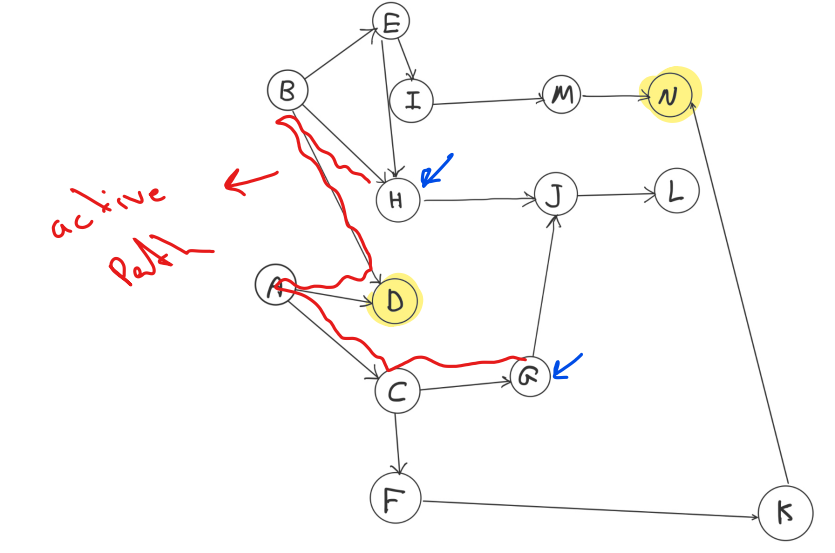
\includegraphics[width=\textwidth]{assets/1a.png}
\end{figure}

\subsection{}
صحیح
\begin{figure}[H]
    \centering
    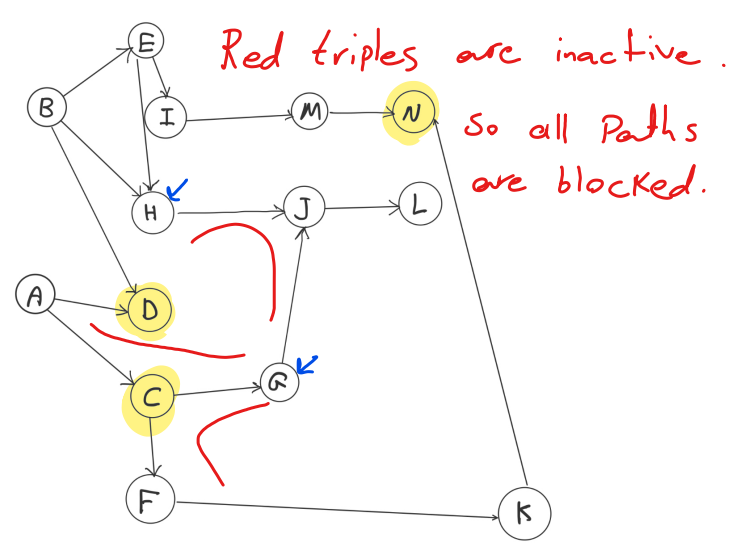
\includegraphics[width=\textwidth]{assets/1b.png}
\end{figure}

\subsection{}
غلط
\begin{figure}[H]
    \centering
    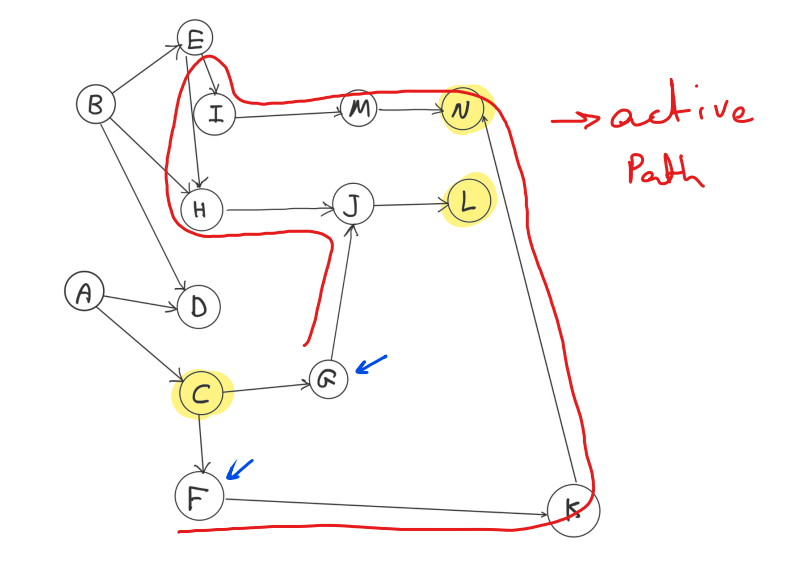
\includegraphics[width=\textwidth]{assets/1c.png}
\end{figure}

\subsection{}
غلط
\begin{figure}[H]
    \centering
    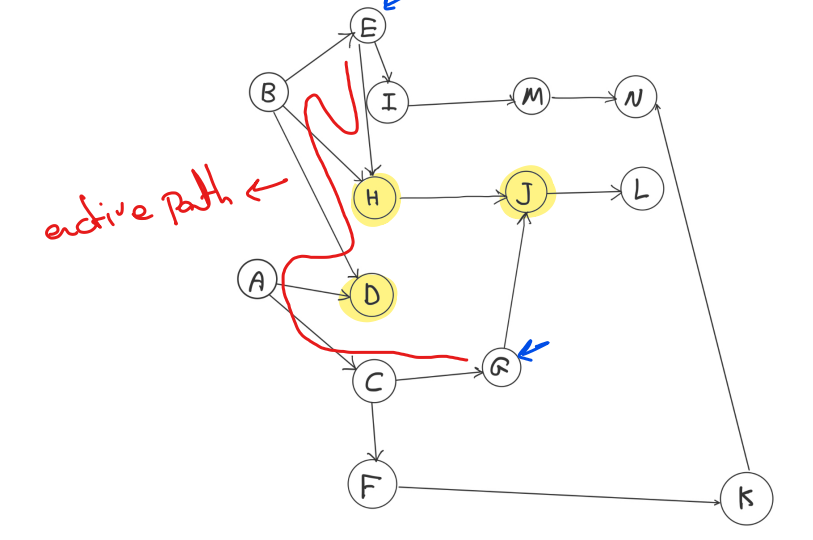
\includegraphics[width=\textwidth]{assets/1d.png}
\end{figure}

\section{}
\subsection{}
\begin{figure}[H]
    \centering
    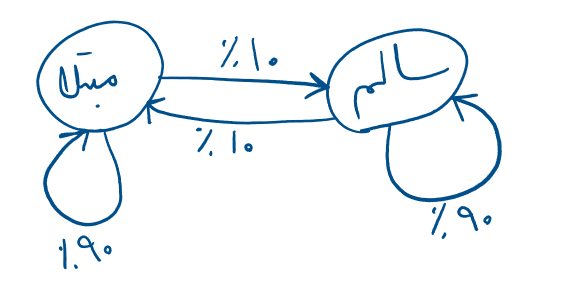
\includegraphics[width=\textwidth]{assets/2a.png}
\end{figure}
\begin{gather*}
    \mathbb{E}[heal] = 0.9 (\mathbb{E}[heal] + 1) + 0.1 \\
    \Rightarrow 0.1 \times \mathbb{E}[heal] = 1 \\
    \Rightarrow \mathbb{E}[heal] = 10
\end{gather*}

\subsection{}
\begin{figure}[H]
    \centering
    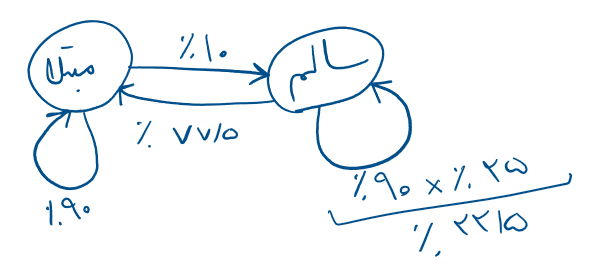
\includegraphics[width=\textwidth]{assets/2b.png}
\end{figure}

\subsection{}
\begin{figure}[H]
    \centering
    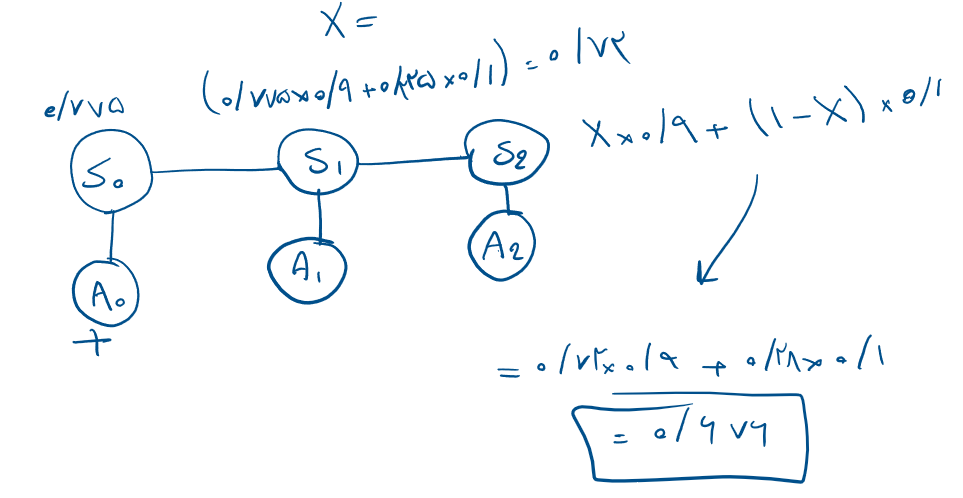
\includegraphics[width=\textwidth]{assets/2c.png}
\end{figure}

\subsection{}
\begin{figure}[H]
    \centering
    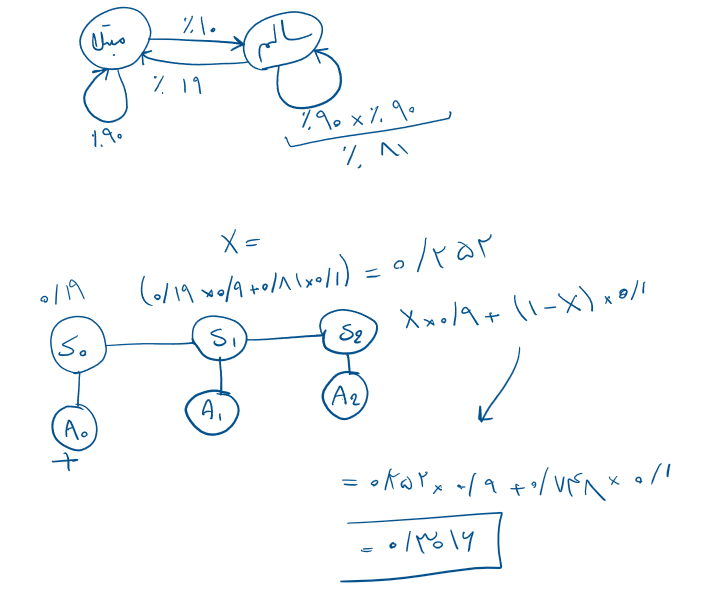
\includegraphics[width=\textwidth]{assets/2d.png}
\end{figure}

\section{}
\subsection{}
\begin{gather*}
H(X) = -\sum_{i=1}^{k} P(X = x_i) \log_2 P(X = x_i) \\
IG(X_i) = H(Y) - H(Y|X_i) \\
H(Y) = -(\frac{4}{6} * \log_2 \frac{4}{6} + \frac{2}{6} \times \log_2 \frac{2}{6}) = 0.38 + 0.52 = 0.9 \\
H(Y|X) = -\sum_{j=1}^{v} P(X = x_j) \sum_{i=1}^{k} P(Y = y_i | X = x_j) \log_2 P(Y = y_i | X = x_j) \\
H(Y|X_1) = -(\frac{3}{6} (0 \log_2 0 + 1 \log_2 1) + \frac{3}{6} (\frac{2}{3} \log_2 \frac{2}{3} + \frac{1}{3} \log_2 \frac{1}{3})) = 0.45 \\
H(Y|X_2) = -(\frac{2}{6} (0.5 \log_2 0.5 + 0.5 \log_2 0.5) \\ 
+ \frac{4}{6} (0.25 \log_2 0.25 + 0.75 \log_2 0.75)) = 0.87 \\
IG(X_1) = 0.9 - 0.45 = 0.45 \\
IG(X_2) = 0.9 - 0.87 = 0.03 
\end{gather*}
\begin{figure}[H]
    \centering
    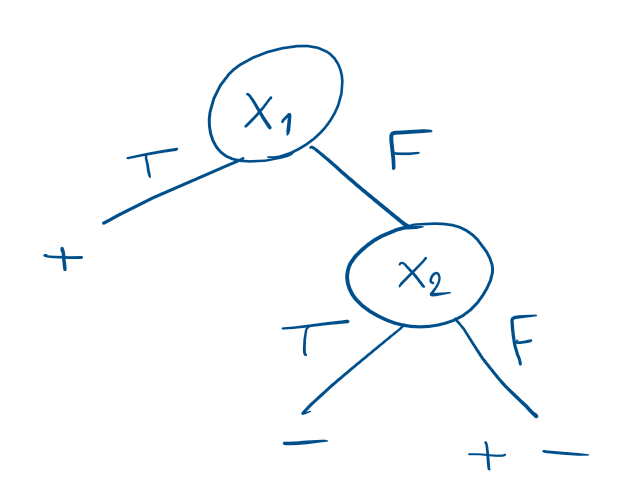
\includegraphics[width=\textwidth]{assets/3a.png}
\end{figure}

\subsection{}
\begin{figure}[H]
    \centering
    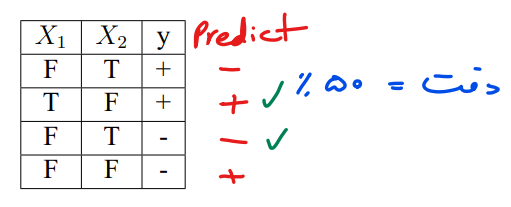
\includegraphics[width=\textwidth]{assets/3b.png}
\end{figure}

\subsection{}
با حذف نود 
\lr{$X_2$}
دقت به اندازه 
\lr{$\frac{1}{4}$}
افزایش پیدا می‌کند. 
\begin{figure}[H]
    \centering
    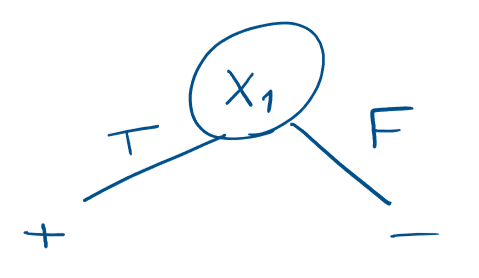
\includegraphics[width=\textwidth]{assets/3c.png}
\end{figure}

\section{}
\subsection{}
\begin{figure}[H]
    \centering
    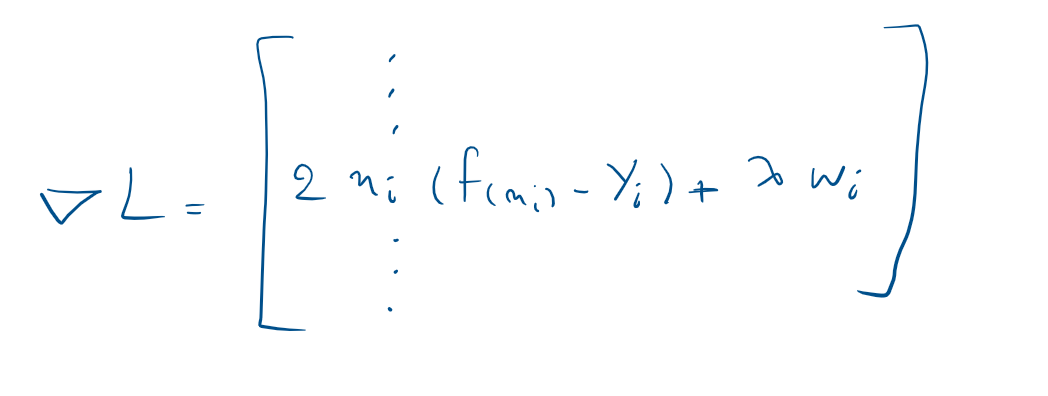
\includegraphics[width=\textwidth]{assets/4a.png}
\end{figure}

\subsection{}
با استفاده از این 
\lr{loss function}
نمودار تابع غیر محدب می‌شود و این باعث می‌شود در مینیمم محلی گیر کنیم. 
همچنین چون توان دو خطا را در نظر میگیریم، ممکن است با تغییر 
یک فیچر مقدار زیادی لاس تغییر کند.

\subsection{}
به دلیل یکنوایی این تابع، برای مسائل کلیسیفیکیشن برای این که به 
اکسترمم گلوبال برسیم می‌توان از آن استفاده کرد. 
\begin{figure}[H]
    \centering
    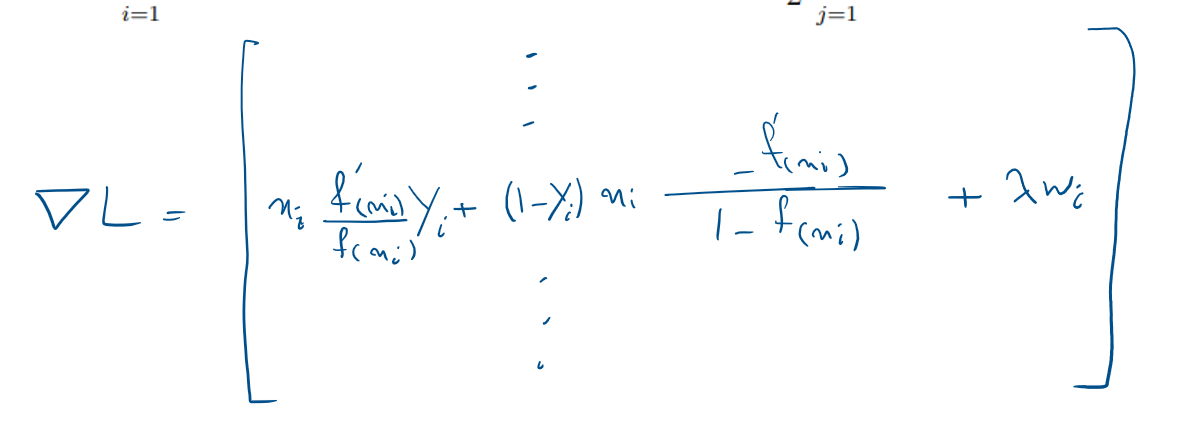
\includegraphics[width=\textwidth]{assets/4c.png}
\end{figure}

\section{}
\subsection{}
\begin{figure}[H]
    \centering
    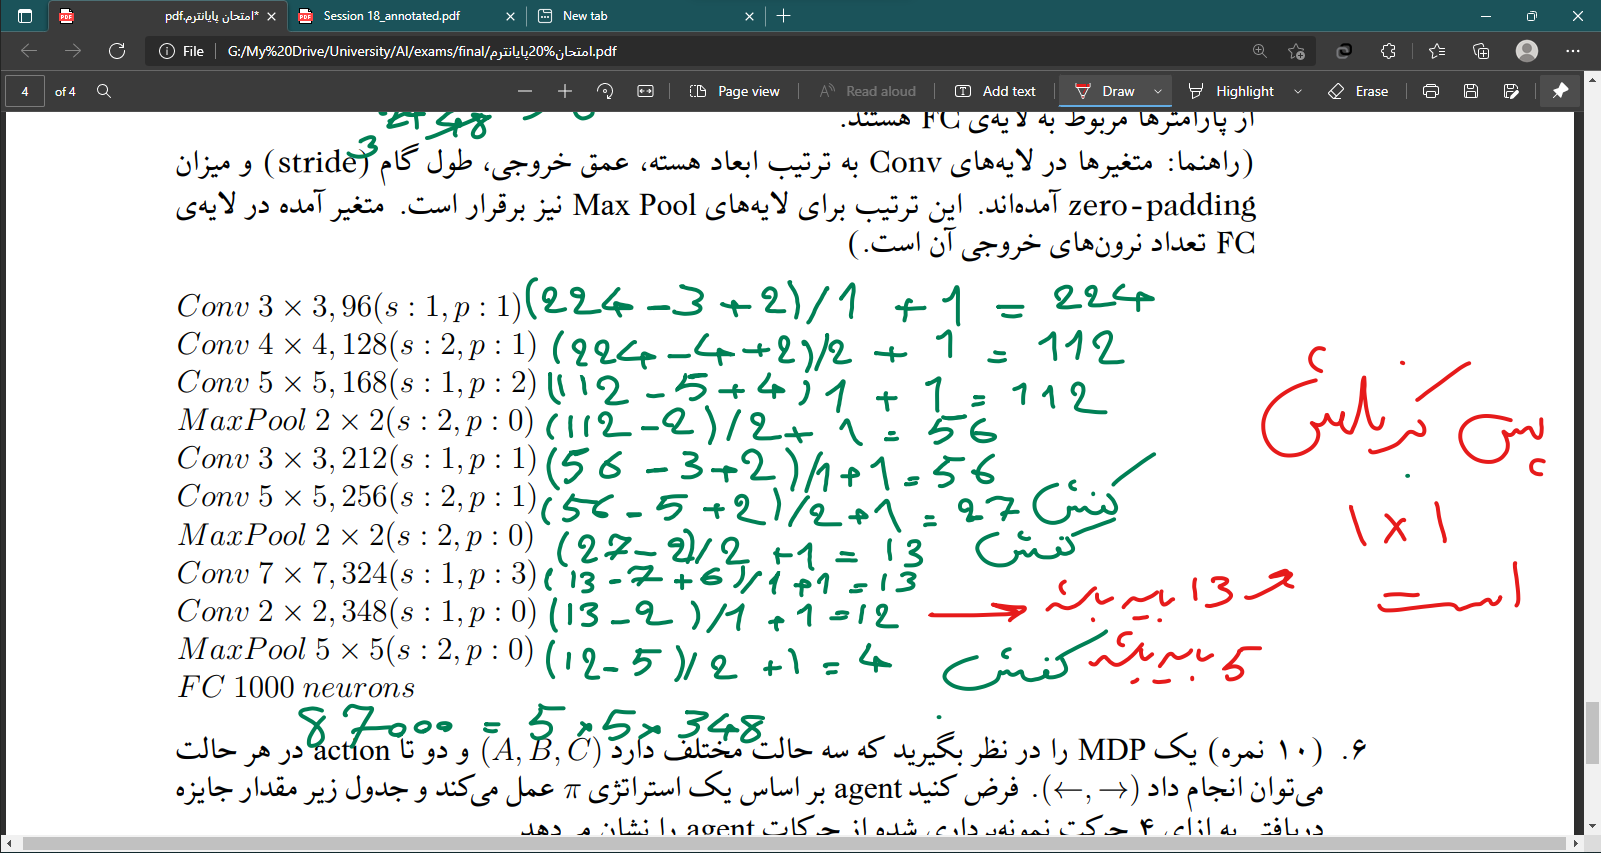
\includegraphics[width=\textwidth]{assets/5a.png}
\end{figure}

\subsection{}
\begin{figure}[H]
    \centering
    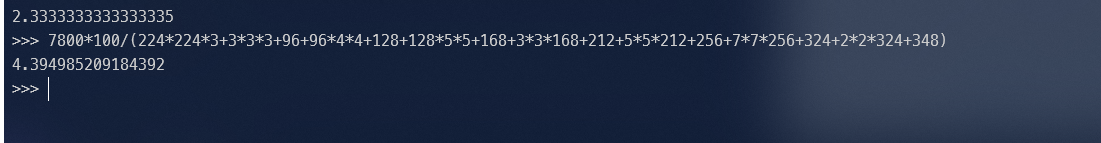
\includegraphics[width=\textwidth]{assets/5b.png}
\end{figure}


\section{}
\begin{figure}[H]
    \centering
    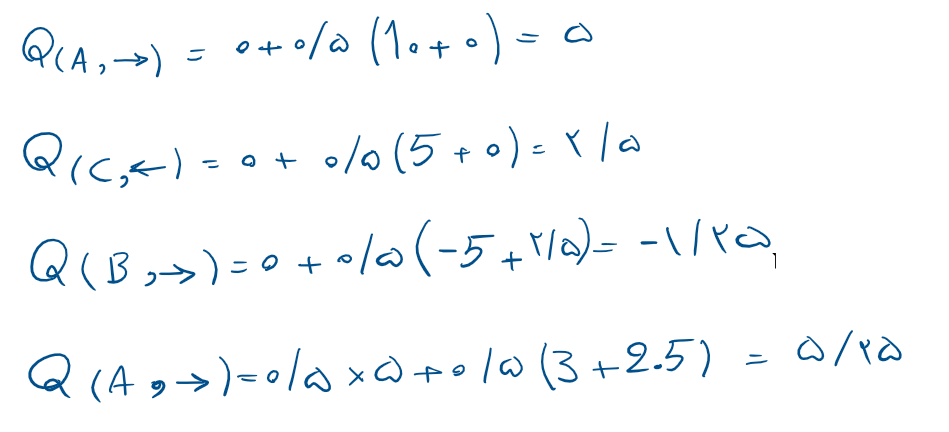
\includegraphics[width=\textwidth]{assets/6.png}
\end{figure}

\end{document}